% Add the option "draft" if needed
\documentclass{statagroupwp}

\usepackage{lipsum}

\title{Long title of the paper}
\journal{GOFCP 2019}
\author{Given Name}{Family Name}{Department of xxx, University of xxx}
\author[*]{Given Name}{Family Name}{Department of xxx, University of xxx}
\author{Given Name}{Family Name}{Department of xxx, University of xxx}
\corrauthor{Name; Address; e-mail: \url{name.surname@university.edu}}
\date{\today}


% Users declarations and packages should be added here
% -- keep them at a minimum, please --




% DOCUMENT

\begin{document}

\maketitle

\begin{abstract}
\lipsum[1]

\keywords{aksa, sakl, askl, askl}
\end{abstract}

\section{Introductory text}

\lipsum[1-2]

\section{Math}

The following math operators are available to the user.

Set of numbers (natural, integer, rational, real, complex):
\[
\Natural, \Integer, \Rational, \Real, \Complex\,.
\]

Statistical operators (expected value, variance, covariance, correlation):
\[
\E, \Var, \cov, \cor
\]

Probability distributions (binomial, Poisson, normal):
\[
\Binom, \Poi, \norm,
\]

Other operators and symbols (big O, define, likelihood function, log-likelihood function, small o, trace of a matric, absolute value, norm, constant $\eu=2.71828\dots$, differential, imaginary unit, indicator function, inverse of a matrix, probability measure, transpose, conjugate transpose):
\[
\bigO, \define, \Lik, \logLik, \smallo, \trace, \abs{\cdot}, \norma{\cdot},
\eu, \diff, \iu, \ind, \inv, \Pr, \T, \HH
\]

System of equations:
\[
\begin{sistema}
ax+by+c =0\\
a'x+b'y+c'=0
\end{sistema}
\]

\noindent\textbf{\em User-defined operators, commands and environments should be avoided, if not necessary.}


\begin{figure}[t]
\centering
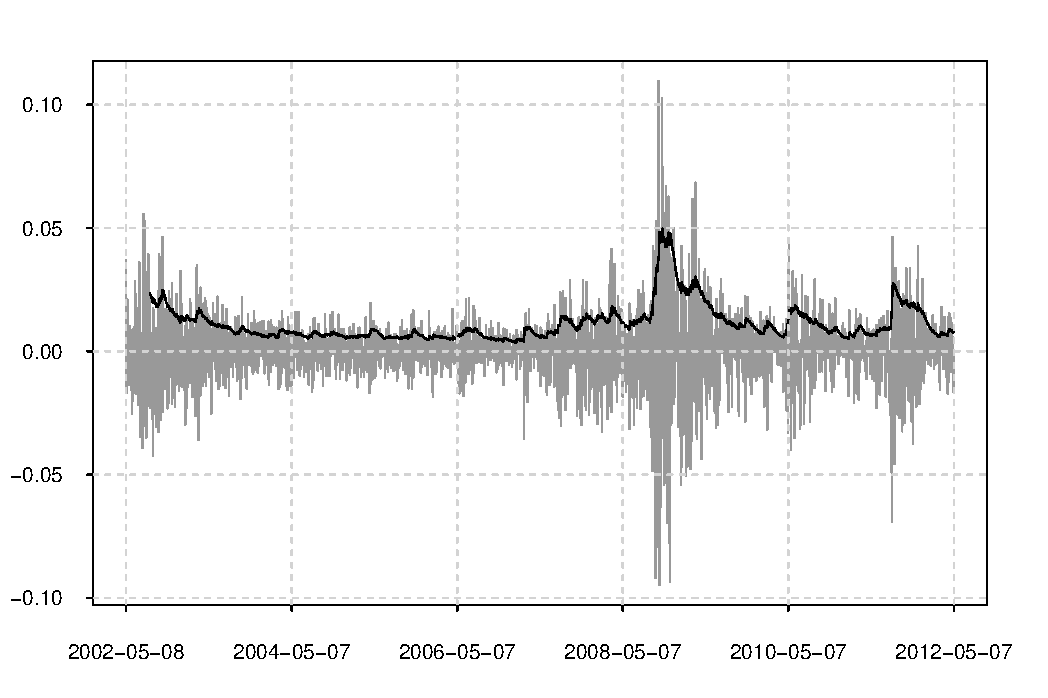
\includegraphics[scale = 0.7]{figures/EWMA}
\caption{aklnsal sa}
\label{fig:coord_y}
\end{figure}


\begin{table}[t]
\centering 
\caption{Nulla malesuada porttitor diam. Donec felis erat, congue non, volutpat at, tincidunt tristique, libero. Vivamus viverra fermentum felis. Donec nonummy pellentesque ante. Phasellus adipiscing semper elit. Proin fermentum massa ac quam.} 
\label{tab:regression} 
\begin{tabular}{@{} l *{4}{d{2.5}} @{}} 
\toprule
 & \multicolumn{4}{c}{\textit{Dependent variable:}} \\ 
\cmidrule(l){2-5}
 & \multicolumn{2}{c}{Trainee} & \multicolumn{2}{c}{Unemployed} \\ 
 & \multicolumn{2}{c}{(1)} & \multicolumn{2}{c}{(2)} \\ 
\midrule
  Constant & -2.494^{***} & (0.197) & -1.910^{***} & (0.158) \\[0.4em] 
  Female & 0.387^{***} & (0.129) & 0.448^{***} & (0.107) \\[0.4em] 
  Low final score & 0.233 & (0.149) & 0.230^{*} & (0.124) \\ 
  High final score & -0.324^{**} & (0.160) & -0.158 & (0.129) \\[0.4em] 
  Short duration & 0.266^{*} & (0.154) & -0.255^{**} & (0.127) \\ 
  Long duration & 0.029 & (0.160) & -0.146 & (0.124) \\[0.4em] 
\bottomrule
\textit{Note:}  & \multicolumn{4}{r}{$^{*}$p$<$0.1; $^{**}$p$<$0.05; $^{***}$p$<$0.01}
\end{tabular} 
\end{table}

\section{Bibliography}


Text citation \cite{gelfand2003}, parenthesis \citep{gelfand2003} citation.



\bibliography{biblio}

\end{document}
